% \documentclass{template/socthesis}
\documentclass[12pt, a4paper]{article}

\usepackage[utf8]{inputenc}
\usepackage[english,shorthands=off]{babel}

% \usepackage[T1]{fontenc} % výstupní kódování
\usepackage{subcaption}
\usepackage{amsmath}
\usepackage{enumitem}
\usepackage{hyperref} % reference
\usepackage{gensymb} % balíček symbolů
\usepackage{booktabs}

\usepackage[toc,page]{appendix}
\usepackage{color} % balíček pro obarvování textů
\usepackage{xcolor}  % zapne možnost používání barev, mj. pro \definecolor
\definecolor{mygreen}{RGB}{0,150,0} % nastavení barev odkazů
\usepackage{listings} % balíček pro formátování zdrojových kódů
\usepackage{multirow}
\usepackage{pifont}
\usepackage{pdfpages}
\usepackage{parskip}
\usepackage[margin=25mm]{geometry}
\usepackage[backend=bibtex]{biblatex}
\usepackage[author=,status=draft]{fixme} % vkládání poznámek
% dva módy (status): draft (poznámky se zobrazují v PDF) / final (poznámky se nezobrazují v PDF)



\newcommand{\cmark}{\textcolor{green}{\ding{51}}}%
\newcommand{\xmark}{\textcolor{red}{\ding{55}}}%

\lstset { %
    language=C++,
    backgroundcolor=\color{black!5}, % set backgroundcolor
    basicstyle=\footnotesize,% basic font setting
}

\setlist[itemize]{parsep=1pt}

\addbibresource{text.bib} % soubor s bibliografií
% \nocite{*}


% hinty k používání balíčků hyperref, url, hyperlink a hypertarget
% \usepackage{hyperref} % balíček pro hypertextové odkazy
% \url{www.odkaz.cz}
% \href{http://www.odkaz.cz}{Text který bude jako odkaz}
% \hyperlink{label}{proklikávací_text} - odkaz na text
% \hypertarget{label}{cíl_odkazu} - cíl odkazu
\title{Integration into Industry 4.0}
\author{Jakub Andrýsek}
\date{}

\begin{document} % konec preambule dokumentu

\maketitle

% #########################################################################################
\section*{Abstract}
I designed a production monitoring system that can record measured data and submit them from machines to a server via the wireless network in real-time.



% #########################################################################################
\section*{Introduction}

This project \emph{Integration into Industry 4.0} deals with a design of a monitoring system for production machines and its deployment in ROTEX Vysočina s.r.o.
This company is making socks, operates daily in two shifts and produces over a hundred and twenty-five thousand pairs of socks monthly.


In the company, there are 25 sock‑knitting machines, which are managed by three operators. The job of an operator consists of checking finished socks and fixing the machines.

The system is internally called iSocks IoT.
The goal of the system is to count the number of finished socks, measure for how long and how often the machines are in error state and compare the performance of different shifts.
It should also provide a summary of the current production to the company management.

In the past, the company had no data about the speed of the knitting machines, the daily production, or the amount of time the machines spent knitting.
My system solves this problem and provides an easy, user-friendly interface, where the user can easily see all these data in charts and tables.

\newpage


% #########################################################################################
\section*{Aims}

This project aims to design a system for automatic monitoring of production machines and their deployment into practice.
The system was designed as a universal platform for monitoring production machines, with the primary focus on sock knitting machines.

The goal of this project was to design a system that:

\begin{itemize}
    \item automatically counts finished socks
    \item online reports machine failures and determines the total failure rate of the machines
    \item compares the efficiency of each working shift
    \item monitors the production process
    \item replaces the monotonous part of operator's job
    \item speeds up and effectively improves the production
    \item reduces the error rate
\end{itemize}


% #########################################################################################
\section*{Materials and methods}

The system consists of a sensor part, a server, and a support server.
The sensor part is built on a circuit board with a microcontroller.
The sensor is connected to the sock knitting machine and sends measured data to the server.
The server receives data from the sensors, processes them, and displays them to the user.
The support server is responsible for updating and checking the correct operation of the sensors.

The system was designed as a universal platform for monitoring production machines with a primary focus on sock knitting machines.
The actual deployment of this system took place in the company ROTEX Vysočina s.r.o. focused on the production of socks.
I deployed my system on ten sock knitting machines, which were operating for 20 months.
During this time, the system recorded over one million finished socks.
This system in the company ROTEX monitors the number of finished socks, how long and how often was each machine stopped, and compares the different shifts.


\begin{figure}[t]
    \centering
    \includegraphics[width=0.7\textwidth]{img/V2-uchyceni.png}
    \caption{Sensor on the machine}
    \label{fig:SenzorNaStroji}
\end{figure}

% #########################################################################################
\subsection*{Sensors}

Sock knitting machines are older devices without internet support.
I had to develop my own sensors for the measurements that acquire data from the electrical components on the knitting machines and send them to the server via a WiFi connection.

Sensors iSocks IoT were designed to be easily connected to existing sock knitting machines and to connect them to the central control system.
Another requirement was to not affect the machine in any way when the sensor is inactive, so the company can operate as usual in case of any problems with the system.

Sensors are built on an ESP32 microcontroller, which provides enough performance and WiFi connectivity.
Each of those sensors has its unique number under which it sends the measured data to the server.
The sensor is powered from 5 or 24 V and has a consumption of 120 mA (on 5 V).

\begin{figure}[t]
    \centering
    \includegraphics[width=0.7\textwidth]{img/oba.png}
    \caption{Sensors: first version on the left, second version on the right}
    \label{fig:dveVerze}
\end{figure}

On each sensor, there are two optocouplers connected to the knitting machine indication diodes.
From one diode, the machine stop is sensed to calculate the time in error state and from the other diode the number of socks knitted is obtained.

The whole measuring and counting system is built using these two LEDs.
Additionally, the sensor has two user buttons, used to set a unique ID of the sensor.
There are two coloured LEDs for direct state indication on the board.

The main visual role is provided by the LCD display, which shows the operators basic machine data.
The wireless connection and sensor number are listed at the top.
In the middle, the number of socks knitted and, in the event of a machine stoppage, the downtime is displayed to the operator in large letters.
This data is prominently displayed on each machine to alert the operator that repair is needed.
The last new feature I have programmed into the sensors is the display of the average sock knitting speed per hour.
We encounter this kind of speed measurement every day in a car, for example, and the operator can quickly calculate the time to finish a job from it.

The sensor is mounted to the machine using compact 3D printed box, which I have designed in Fusion 360 and printed on the FDM 3D printer.

\begin{figure}[htbp]
    \centering
    % \includegraphics[scale=0.5]{DATASHEET/Pletacka_board_v2.pdf}
    \includegraphics[width=\textwidth]{DATASHEET/Pletacka_board_v2.pdf}
    \caption{Schematic of the sensor}
    \label{fig:Schemav1}
\end{figure}

% #########################################################################################
\subsection*{Web server}

The server is an integral part of the system. It takes care of receiving the measured data, processing them and then displaying them to the user.
The server itself runs on a Raspberry Pi 4 Model B microcomputer.

The device runs the Raspberry Pi OS operating system with a graphical interface.
The website runs on an Apache2 HTTP server and PHP 8.0.
As a database system I use MariaDB.
The server runs locally within the company on a secure network, which makes the system fast and independent of the internet connection.

To connect to the web server you can open a local company link \newline\href{http://iSocks.lan}{iSocks.lan}.
The user is then presented with an initial overview page with coloured bubbles representing each knitting machine.
The colour of the bubbles indicates the current state of the machine.
The user can thus very quickly find out the current condition of the knitting machines without having to visit the knitting factory.
In addition to the colour, the bubble also displays text, which shows the number of socks knitted and if the machine stops and turns red, the text changes to the time the machine is stopped for.



\begin{figure}[t]
    \centering
    \includegraphics[width=0.9\textwidth]{img/Uvod.png}
    \caption{Home page}
    \label{fig:webUvod}
\end{figure}

The next section of the interface are the Sensor Reports generated for each knitting machine.
Here the user is shown the data in different time reports.
For easy comparison of data between two shifts, these data are displayed side by side.
Underneath the numerical reports, there are pre-generated long-term graphs, see \ref{fig:webSenzory}.

Each sensor uses five database tables. The first is used to store raw data, while the remaining tables store automatically generated aggregated reports.
These are used to quickly plot graphs and calculate long-term data.
The sensor records the knitted sock and sends the measured data to the web server via REST API, which checks it and stores it in the database for the specific sensor.
Each database record contains the machine number, unique event ID, measured state and event time.

% \includepdf[pages=-, scale=0.6, pagecommand={}]{DATASHEET/Pletacka_board_v2.pdf}


\begin{figure}[t]
    \centering
    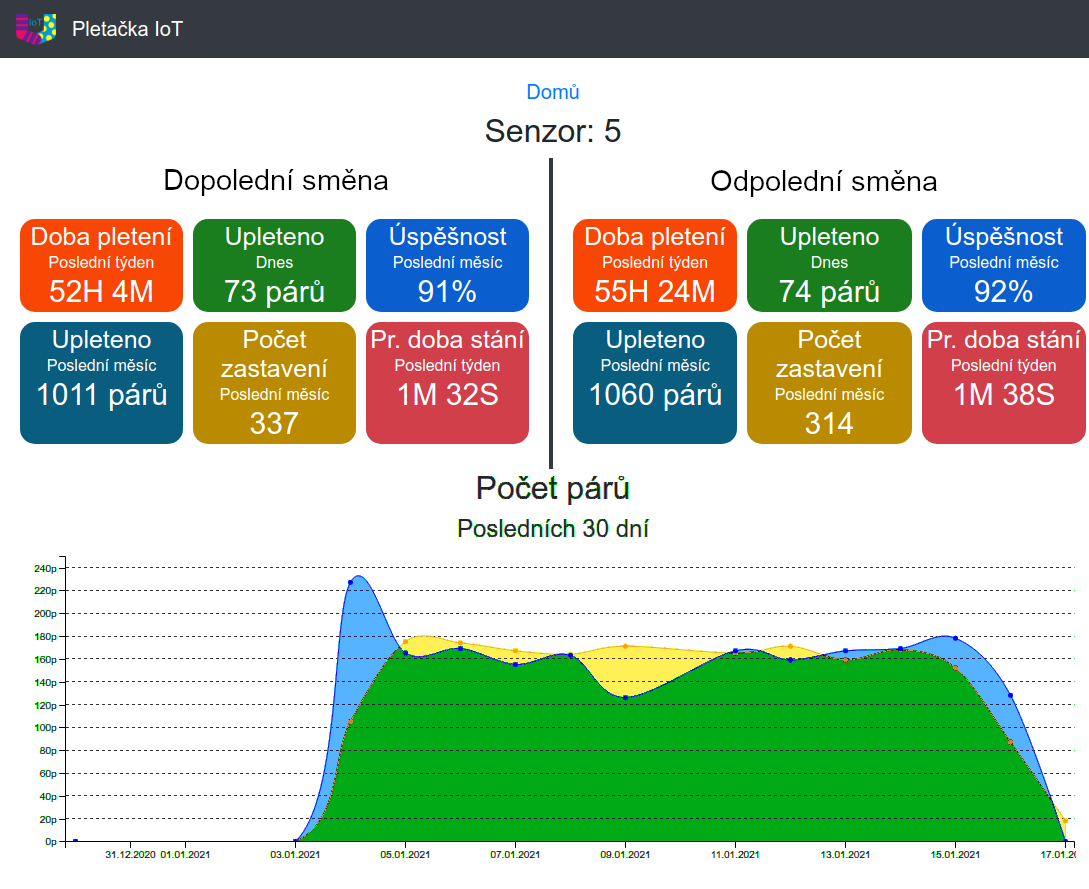
\includegraphics[width=0.6\textwidth]{img/prehled.png}
    \caption{Sensor charts}
    \label{fig:webSenzory}
\end{figure}


% #########################################################################################
\subsection*{Support server}

The support server was created as an extension for the sensors.
The server is programmed in Python and runs on a Raspberry Pi together with a web server.\newline

The main task of this server is to detect switched on sensors.
The server runs the so-called Watchdog.
It is a periodic loop that waits for a message from a sensor every four seconds.
With this message, the sensor reports that it is on. If such a message does not arrive within ten seconds, the sensor is declared off and marked as inactive in the database.

\newpage
% #########################################################################################
\subsection*{How iSocks IoT works}

The previous chapters described the parts of the iSocks IoT system.
In this chapter, the whole system will be described as a single unit.

The first as well as the most important part is data acquisition using sensors.
As soon as a sensor detects any change, it immediately sends this message to the server.
The sending is done through the sensor API, where the sensor is first authenticated and then the status is written to the database for the corresponding sensor.
After writing to the database the server returns a confirmation message.

The second step is to process the raw data from the database.
For this purpose, a selection API is running on the server, which is automatically started at a set time.
It is used to generate broader data aggregations, hourly, daily, monthly and yearly.
These aggregations are then stored in the database for the sensor.
The generation of this data is mostly done at night when the server is the least busy.

The last step is to display the data to the user.
This is the only part of the system that a normal user is going to see and control.
Therefore, it is necessary to make the display as fast and user-friendly as possible.
To make the display fast, pre-generated aggregations are used, to which the real-time data are appended and the entire result is displayed to the user.

% \begin{figure}[t]
%     \centering
%     \includegraphics[width=0.9\textwidth]{img/Princip.png}
%     \caption{Data processing}
%     \label{fig:princip}
% \end{figure}


% #########################################################################################
\subsection*{Testing}

I have been developing the entire system since February 2020.
The first small tests were performed in May 2020, but the full system was tested in the summer of 2020 and in the Autumn of 2020.
From then on the system is fully deployed  and maintained in the company.

\begin{figure}[t]
    \centering
    \includegraphics[width=0.7\textwidth]{img/pletarna.png}
    \caption{Machines in the factory}
    \label{fig:MachinesInTheFactory}
\end{figure}

% #########################################################################################
\newpage
\section*{Results and discussion}

All the goals of the project set at the beginning were achieved.
The old (yet functional) knitting machines were transformed into modern ones with online monitoring using my system, at a fraction of the cost.
The system improved production time, reduced operator time and introduced a detailed overview of the product including a comparison of changes in production.
The system reduced the production cost by minimizing the manufacturing time and downtime.

As of June 20 2021, the system is deployed on ten knitting machines and has already recorded over one million knitted socks without a sensor malfunction.

A big advantage of this system is that it can compare the work shifts of employees and thus the company management can see the differences between them.

Thanks to this project, I learned how to design circuit boards, work with electronic components and tried different programming methods.
I also learned how to program in PHP and create complex web systems.

In the future, I would like to extend this system to all machines and cover the entire production.
I would also like to continue to improve the web application. I plan to expand it with other functions, such as exporting data to spreadsheets.

All source code and DPS of the project are available at \url{https://github.com/Pletacka-IoT} under the MIT license.


\newpage

\appendix


\end{document}

% Uprava na tvrde mezery "\b([aiouksvz]) " (i s tou mezerou na konci) => "$1 "
